\documentclass[en]{../../../eplsummary}

\usepackage{../../../eplcommon}
\usepackage{../../../eplcode}
\usepackage{float}
\lstset{language=Java, basicstyle=\rm\small\ttfamily}

\hypertitle[']{Algorithmique et structures de données}{5}{LSINF}{1121}
{Antoine Paris}
{Pierre Schauss}

% TODO
% - translate everything to english
% - improve a lot section on sorting

\section{Piles, files et listes chaînées}
\subsection{Listes chaînées}
\paragraph{Définition} Une \textit{liste chaînée}
est une structure de données récursive qui est soit
vide (\textit{null}) soit une référence vers un
noeud contenant une donnée générique et une référence
vers une liste chaînée.

Pour définir un noeud, on utilise une classe imbriquée :

\begin{lstlisting}
private class Node {
	private Item item;
	private Node next;
}
\end{lstlisting}

Une liste chaînée permet, si on possède un lien vers
le premier et le dernier élément de réaliser les
opérations suivantes en un temps indépendant de la
taille de la liste :

\begin{itemize}
	\item Insérer un élément au début ;
	\item Supprimer un élément au début ;
	\item Insérer un élément à la fin.
\end{itemize}

Pour pouvoir effectuer des insertions/suppressions
arbitraires efficacement, il faut utiliser des listes
doublement chaînées (chaque noeud possède deux liens,
un dans chaque direction).

Les implémentations de \lstinline{Stack}, \lstinline{Queue}
et \lstinline{Bag} reposent sur les listes chaînées. Grâce
à ces dernières, l'espace mémoire requis est proportionnel
au nombre d'items dans la collection et le temps requis
par opération est toujours indépendant de la taille de la
collection (ce ne serait pas le cas en utilisant des tableaux
par exemple).

\subsection{Stack}
Le principe de fonctionnement d'une stack est illustré à la figure
\ref{fig:stack}.

\begin{figure}[ht]
	\centering
	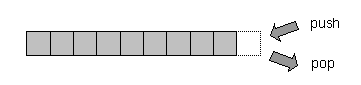
\includegraphics[scale=1.0]{img/stack.png}
	\caption{Illustration du fonctionnement d'une Stack LIFO.}
	\label{fig:stack}
\end{figure}

\lstinputlisting{code/Stack.java}

\subsection{Queue}
Le principe de fonctionnement d'une queue est illustré à la figure
\ref{fig:queue}.

\begin{figure}[ht]
	\centering
	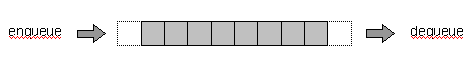
\includegraphics[scale=1.0]{img/queue.png}
	\caption{Illustration du fonctionnement d'une Queue FIFO.}
	\label{fig:queue}
\end{figure}

\lstinputlisting{code/Queue.java}

\subsection{Bag}
Un bag est simplement une stack sans méthode \lstinline{pop()}.

\section{Algorithmes de tri}
Le but du jeu ici est de trier des tableaux d'items contenant
chacun une clé en suivant un ordre bien particulier (le plus
souvent numérique ou alphabétique). La notion de clé est inclue
dans un mécanisme propre à Java, l'interface \lstinline{Comparable}
(et notamment la méthode \lstinline{compareTo}).

On distingue deux types d'algorithmes de tri, les algorithmes
\textbf{en place} qui n'utilisent pas (ou quasi pas) de mémoire
supplémentaire et ceux qui nécessitent assez de mémoire
supplémentaire pour garder une copie du tableau à trier en
mémoire.

Dans les algorthimes de tri présentés dans cette section,
on utilise le template suivant.

\lstinputlisting{code/SortTemplate.java}

\subsection{Selection Sort}
\subsubsection{Principe}
Le tri par sélection est un des plus simple. Il fonctionne
comme suit : premièrement, trouver l'élément le plus petit
du tableau et l'échanger avec le premier élément, ensuite
trouver le deuxième élément le plus petit du tableau et
l'échanger avec le deuxième élément, et ainsi de suite.
La traduction en Java est immédiate.

\subsubsection{Implémentation}
\lstinputlisting{code/Selection.java}

\subsubsection{Propriétés}
\paragraph{Le temps d'éxécution est indépendant de l'entrée}
L'algorithme mettra autant de temps à trier à tableau déjà
trié qu'un tableau aléatoirement ordonné.

\paragraph{Mouvement minimal}
Le nombre d'échange est une fonction linéaire de la taille
du tableau à trier ($N$ échanges sont effectués). 

\subsubsection{Complexité}
Dans tous les cas $\frac{N^2}{2}$ comparaisons et $N$ échanges.

\subsection{Insertion Sort}
\subsubsection{Principe}
C'est l'algorithme qu'on utilise en général pour trier
ses cartes. On considère une carte à la fois, et on
l'insère à sa place parmis les cartes déjà triées. La
seule différence est qu'ici il faut faire de la place
pour insérer l'item considéré à sa position, on doit
donc décaler tout les items plus grand que lui d'une
position vers la droite.

\subsubsection{Implémentation}
\lstinputlisting{code/Insertion.java}

\subsubsection{Propriétés}
Contrairement au tri par sélection, le temps d'éxécution
du tri par insertion est dépendant de l'entrée, il est par
exemple \textbf{excellent pour des tableaux presque triés}.

C'est également une méthode correcte pour de très petits
tableaux.

\subsubsection{Complexité}
Dans le pire cas, $\frac{N^2}{2}$ comparaisons et
$\frac{N^2}{2}$ échanges.

\subsection{Shell Sort}
\subsubsection{Principe}
Le shellsort est juste une simple extension du tri
par insertion. Dans le tri par insertion, les échanges
n'impliquent que des éléments adjacents, les items ne
peuvent donc se déplacer que d'un élément à la fois.
Le shellsort gagne en rapidité en autorisant des échanges
d'éléments éloignés dans le tableau.

\paragraph{Tableau $h$-trié} un tableau $h$-trié ($h$-sorted
array) est un tableau dont tous les éléments séparés
de $h$ positions sont triés.

\subsubsection{Implémentation}
Concrètement, l'algorithme s'implémente en utilisant le
tri par insertion pour obtenir successivement des 
tableaux $h$-triés avec $h$ décroissant.

\lstinputlisting{code/Shell.java}

\subsubsection{Propriétés}
Lorsqu'un tableau $h$-trié est $k$-trié, il reste
$h$-trié.

\subsubsection{Complexité}
Un peu moins quadratique, $N^{\frac{4}{3}}$, $N^{\frac{5}{4}}$
ou $N^{\frac{6}{5}}$ dans le pire cas.

\subsection{Mergesort}
Le principe du tri par fusion est assez simple : pour trier
un tableau, diviser le en deux moitiés, trier chaque moitié
(récursivement) et ensuite fusionner les résultats.

La complexité des algorithmes de tri par fusion est
logarithmique en $N\log N$. Le tri par fusion est
un algorithme de tri basé sur des comparaisons
asymptotiquement optimal (on ne peut pas faire mieux).

Les deux implémentations du tri par fusion vues ici
se base sur la méthode \lstinline{merge} suivante :

\lstinputlisting{code/mergeMethod.java}

\subsubsection{Top-down mergesort}
Ici, on divise le problème en sous-problèmes et on les résout
récursivement. 

\lstinputlisting{code/Merge.java}

\begin{figure}[ht]
	\centering
	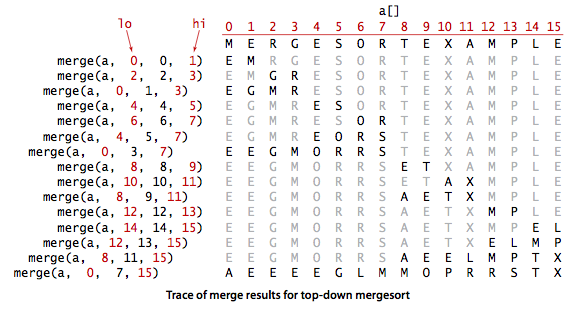
\includegraphics[scale=0.5]{img/mergesortTD.png}
	\caption{Trace des résultats de merge pour le top-down mergesort.}
\end{figure}

\subsubsection{Bottom-up mergesort}
Ici, on construit des petites solutions que l'on rassemble
pour en former des plus grandes à chaque fois. 

\lstinputlisting{code/MergeBU.java}

\begin{figure}[ht]
	\centering
	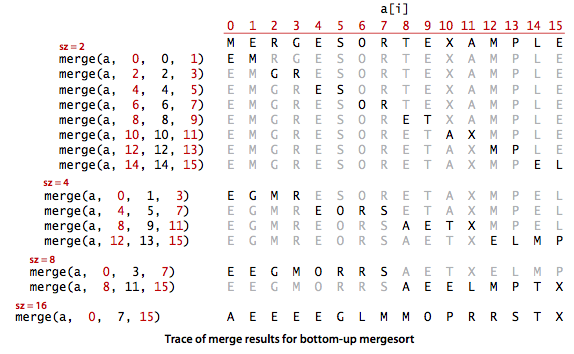
\includegraphics[scale=0.5]{img/mergesortBU.png}
	\caption{Trace des résultats de merge pour le bottom-up mergesort.}
\end{figure}

C'est la méthode à privilégier pour trier une liste chaînée.

\subsection{Quicksort}
\subsubsection{Principes}
Le tri rapide est probablement le plus utilisé, et ce pour
les deux raisons suivantes : il est en place et s'éxécute
en un temps proportionnel à $N \log N$.
Il fonctionne selon le principe du \textit{diviser pour
mieux régner}. Il partitionne le tableau en deux parties
et les trie ensuite indépendemment comme illustré sur
la figure \ref{fig:quicksort-overview}

\begin{figure}[ht]
	\centering
	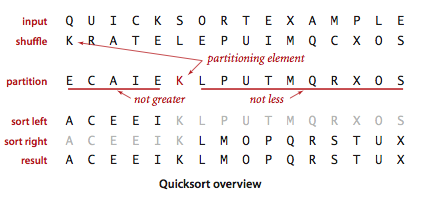
\includegraphics[scale=0.7]{img/quicksort-overview.png}
	\caption{Quicksort overview.}
	\label{fig:quicksort-overview}
\end{figure}

L'algorithme de partionnement doit réarranger le tableau pour que
les 3 conditions suivantes soient vérifiées :

\begin{itemize}
	\item L'entrée \lstinline{a[j]} est à sa position finale pour
	un certain $j$ ;
	\item Les entrées \lstinline{a[lo..j-1]} sont inférieures ou
	égales à \lstinline{a[j]} ;
	\item Les entrées \lstinline{a[j+1..hi]} sont supérieures ou
	égales à \lstinline{a[j]}.
\end{itemize}

Ces 3 conditions sont résumées sur la figure \ref{fig:part-overview}.

\begin{figure}[ht]
	\centering
	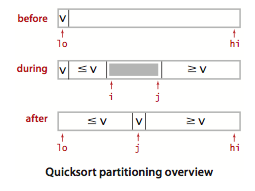
\includegraphics[scale=0.7]{img/partitioning-overview.png}
	\caption{Partioning overview.}
	\label{fig:part-overview}
\end{figure}

\subsubsection{Implémentation}
La trace du code suivant se trouve à la figure \ref{fig:part-trace}

\lstinputlisting{code/Quick.java}

\begin{figure}[ht]
	\centering
	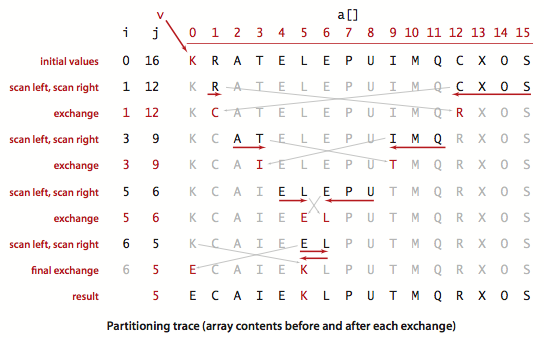
\includegraphics[scale=0.5]{img/partitioning.png}
	\caption{Partioning trace.}
	\label{fig:part-trace}
\end{figure}

\subsubsection{Complexité}
Dans le pire cas, le tri rapide a une complexité quadratique.
Il est possible d'éviter ce pire cas en mélangeant aléatoirement
le tableau avant de le trier (cela fait du tri rapide un
algorithme \textit{randomisé}).

Dans le cas moyen, le tri rapide a une complexité en $\mathcal{O}(n\log(n))$.

\subsection{3-way quick sort}
\subsubsection{Principes}
Si le tableau à trier contient beaucoup d'éléments dupliqués (voir \textit{Dutch
National Flag problem}), il est possible d'atteindre une complexité
linéaire en modifiant un peu le tri rapide.

L'idée est d'utiliser 3 partitions plutôt que 2, comme indiqué sur
la figure \ref{fig:part3-overview}.

\begin{figure}[ht]
	\centering
	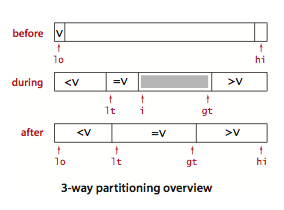
\includegraphics[scale=0.7]{img/partitioning3-overview.png}
	\caption{3-way partioning overview.}
	\label{fig:part3-overview}
\end{figure}

Pour cela, une solution est d'effectuer un simple scan de la gauche
vers la droite dans le tableau en maintenant une variable \lstinline{lt}
tel que \lstinline{a[lo..lt-1]} sont inférieurs à $v$, une variable
\lstinline{gt} tel quel \lstinline{a[gt+1..hi]} sont plus grands que $v$,
une variable $i$ tel que \lstinline{a[lt..i-1]} sont égals à $v$ et
\lstinline{a[i..gt]} n'ont pas encore été examinés.

% TODO : add summary of complexity for sorting algorithms

\subsubsection{Implémentation}
La trace du code suivant se trouve à la figure \ref{fig:part3-trace}

\lstinputlisting{code/Quick3way.java}

\begin{figure}[ht]
	\centering
	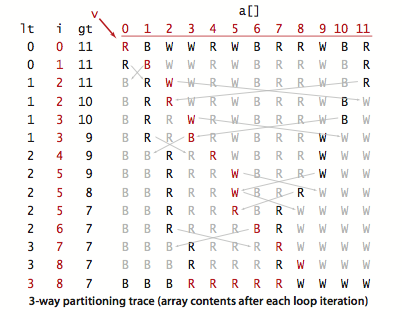
\includegraphics[scale=0.7]{img/partitioning3.png}
	\caption{3-way partioning trace.}
	\label{fig:part3-trace}
\end{figure}

\section{Searching}
\subsection{Symbol tables}
\begin{mydef}
A \textit{symbol table} is a data structure for key-value pairs that
supports two operations: \textit{insert} (put) a new pair into the
table and \textit{search} for (get) the value associated with a given
key.
\end{mydef}

Here we adopt the \textit{associative array abstraction}, where you can
think of a symbol table as being just like an array where keys are
indices and values are array entries.

The API for a generic basic symbol table is given in figure \ref{fig:st-api}.

\begin{figure}[ht]
	\centering
	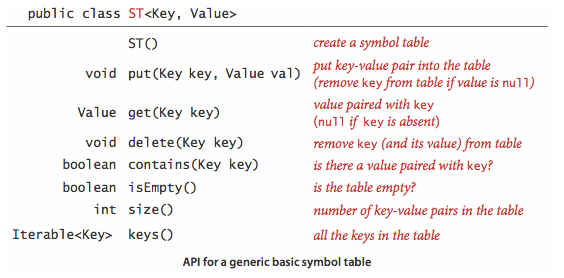
\includegraphics[scale=0.5]{img/symbol-table-api.png}
	\caption{API for a generic basic symbol table.}
	\label{fig:st-api}
\end{figure}

For applications where keys are \lstinline{Comparable}, we usually talk about
\textit{ordered symbol tables}, where keys are kept in order.

The API for a generic ordered symbol table is given in figure \ref{fig:ost-api}.

\begin{figure}[ht]
	\centering
	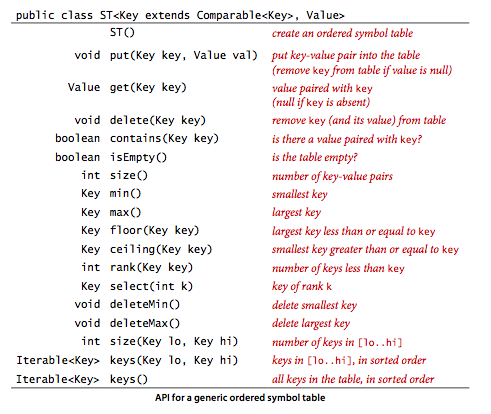
\includegraphics[scale=0.5]{img/ordered-symbol-table-api.png}
	\caption{API for a generic ordered symbol table.}
	\label{fig:ost-api}
\end{figure}

\subsubsection{Sequential search in an unordered linked list}
One straightforward option for the underlying data structure for a
symbol table is a linked list of nodes that contain keys and values.

Implementations of both \lstinline{get()} and \lstinline{put()} consist
of scanning through the list. Hence, it is easy to show that the worst
case is $\mathcal{O}(n)$ for both. In conclusion, a linked-list
implementation with sequential search is too slow to be used to solve
huge problems.

\subsubsection{Binary search in an ordered array}
\begin{lstlisting}
public class BinarySearchST<Key extends Comparable<Key>, Value>
{
\end{lstlisting}

Now, we consider a full implementation of our ordered symbol-table API.
The underlying data structure is a pair of parallel arrays, one for the
keys and one for the values.

\begin{lstlisting}
    public BinarySearchST(int capacity) { 
        keys = (Key[]) new Comparable[capacity]; 
        vals = (Value[]) new Object[capacity]; 
    }
    
    public int size() {
        return N;
    }
\end{lstlisting}

The heart of the implementation is the \lstinline{rank()} method, which
returns the number of keys smaller than a given key. For \lstinline{get()},
the rank tells us precisely where the key is to be found it is in the table.

\begin{lstlisting}
	public Value get(Key key) {
		if (isEmpty()) return null;
		int i = rank(key); 
		if (i < N && keys[i].compareTo(key) == 0) return vals[i];
    		return null;
	} 
\end{lstlisting}

For \lstinline{put()}, the rank tells us precisely where to update the value
when the key is in the table, and precisely where to put the key when the
key is not in the table. We move all larger keys one position to make room
and insert the given key and value into the proper positions in their
respective arrays.

\begin{lstlisting}
	public void put(Key key, Value val)  {
		int i = rank(key);

		if (i < N && keys[i].compareTo(key) == 0) {
			vals[i] = val; return;
		}

		for (int j = N; j > i; j--)  {
			keys[j] = keys[j-1]; vals[j] = vals[j-1];
		}
        
		keys[i] = key; vals[i] = val;
		N++;
	} 
\end{lstlisting}

To find the rank of a given key, we take advantage of the fact that keys
in the array are ordered and use \textit{binary search}. An iterative
implementation of the \lstinline{rank()} method is given below.

\begin{lstlisting}
	public int rank(Key key) {
		int lo = 0, hi = N-1;
		while(lo <= hi) {
			int mid = low + (hi - lo)/2;
			int cmp = key.compareTo(keys[mid]);
			if		(cmp < 0) hi = mid-1;
			else if 	(cmp > 0) hi = mid+1;
			else	 return mid; 		
		}
		
		return lo;	
	}
\end{lstlisting}

Here, it is easy to show that the complexity of binary search
is $\mathcal{O}(n\log(n))$. Unfortunately, insertion is still
to slow : $\mathcal{O}(n)$.

\subsection{Binary search tree}
Here we'll combine the flexibility of insertion in a linked-list
with the efficiency of search in an ordered array.

\begin{mydef}
A \textit{binary search tree} (BST) is a binary tree where each node
has a \lstinline{Comparable} key (and a associated value) and
satisfies the restriction that the key in any node is larger than
the keys in all nodes in that nodes' left subtree and smaller
than the keys in all nodes in that node's right subtree.
\end{mydef}

This restriction is illustrated in figure \ref{fig:bst-anatomy}.
Note that on a binary tree that is not a binary \textit{search}
tree, we don't have this restriction.

\begin{figure}[ht]
	\centering
	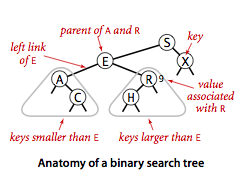
\includegraphics[scale=0.65]{img/bst-anatomy.png}
	\caption{BST anatomy.}
	\label{fig:bst-anatomy}
\end{figure}

\begin{myrem}
It's interesting to note that there are many different BSTs that
represent the same set.
\end{myrem}

\subsubsection{Basic implementation}
\begin{lstlisting}
public class BST<Key extends Comparable<Key>, Value>
{
	private Node root;
\end{lstlisting}

Just as we did for linked lists, we define a private nested class
to define nodes in BSTs.

\begin{lstlisting}
	public class Node {
		private Key key;
		private Value val;
		private Node left, right;
		private int N;
		
		public Node(Key key, Value val, int N) {
			this.key = key; this.val = val; this.N = N;		
		}	
	}
\end{lstlisting}

Each node contains a key, a value, a left and right link and a node
count. This last field facilitates the implementation of various
ordered symbol-table operations.

\begin{lstlisting}
	public int size() {
		return size(root);	
	}
	
	private int size(Node x) {
		if (x == null) return 0;
		else return x.N;	
	}
\end{lstlisting}

Thanks to the recursive definition of a tree, we can implement
the \lstinline{get()} easily in a recursive way.

\begin{lstlisting}
	public Value get(Key key) {
		return get(root, key);	
	}
	
	private Value get(Node x, Key key) {
		if (x == null) return null;
		
		int cmp = key.compareTo(x.key);
		if      (cmp > 0) return get(x.right, key);
		else if (cmp < 0) return get(x.left, key);
		else	 return x.val;
	}
\end{lstlisting} 

The same holds for the \lstinline{put()} method.

\begin{lstlisting}
	public void put(Key key, Value val) {
		root = put(root, key, val);	
	}
	
	private Node put(Node x, Key key, Value val) {
		if (x == null) return new Node(key, val, 1);
		
		int cmp = key.compareTo(x.key);
		if      (cmp > 0) x.right = put(x.right, key, val);
		else if (cmp < 0) x.left = put(x.left, key, val);
		else x.val = val;
		x.N = size(x.left) + size(x.right) + 1;
		return x;
	}
\end{lstlisting}

To get a better understanding of the dynamics of these
recursive implementations, you can think of the code
\textit{before} the recursive calls as happening on the
way \textit{down} the tree. Then, think of the code \textit{after}
the recursive calls as happeing on the way \textit{up} the tree.

Now, let's look at how to delete a node in a BST. This is the most
difficult operation to implement. We choose here to use the
\textit{Hibbard deletion}. With this method, we delete a node
$x$ by replacing it with its \textit{successor}. If $x$ has
a right child, its successor is the node with the smallest
key in its right subtree. This task is accomplished
in 4 steps :

\begin{itemize}
	\item Save a link to the node to be deleted in \lstinline{t} ;
	\item Set \lstinline{x} to point to its successor
	\lstinline{min(t.right)} ;
	\item Set the right link of \lstinline{x} to
	\lstinline{deleteMin(t.right)} ;
	\item Set the left link of \lstinline{x} to \lstinline{t.left}.
\end{itemize}

\begin{lstlisting}
	public void delete(Key key) {
		root = delete(root, key);	
	}
	
	private Node delete(Node x, Key key) {
		if (x == null) return null;
		int cmp = key.compareTo(x.key);
		if      (cmp < 0) x.left = delete(x.left, key);
		else if (cmp > 0) x.right = delete(x.right, key);
		else {
			if(x.right == null) return x.left;
			if(x.left == null) return x.right;
			Node t = x;
			x = min(t.right);
			x.right = deleteMin(t.right);
			x.left = t.left;		
		}	
		
		x.N = size(x.left) + size(x.right) +1;
		return x;
	}
\end{lstlisting}

Even though this method does the job, it has a flaw that might
cause performance problems in some practical situations. The problem
is that the choice of using the successor is arbitrary and not
symmetric. This will cause the BST to become skewed toward the
left on the long term for random deletions and insertions
\footnote{See the last video on 
\url{http://algs4.cs.princeton.edu/32bst/}.}.

\begin{myrem}
Others methods from the API are in the book.
\end{myrem}

\subsubsection{Analysis}
The running times of algorithms on binary search trees depend
on the shapes of the trees, which in turn, depend on the
order in which keys are inserted. In the best case, a tree
with $N$ nodes could be perfectly balanced, with $\log(n)$
nodes between the root and each null links (we call this the
\textit{depth} of a tree). In the worst case
there could be $N$ nodes on the search patch.

% Better to say "proposition" than "property" ? Do I need to change
% eplcommon.sty to add this?
\begin{myprop}
Search hits in BST build from $N$ random keys requires $\sim 2\log N$
(about $1.39\log(n)$) compares, on the average.
\end{myprop}

\begin{myprop}
Insertions and search misses in a BST build from $N$ random
keys require $\sim 2\log N$ (about $1.39\log(n)$) compares on the
average.
\end{myprop}

\begin{myprop}
In a BST, all operations take time proportional to the height of
the tree in the worst case.
\end{myprop}

\subsection{Balanced search tree}
The algorithms in the previous subsection have poor worst-case,
performance. Here we introduce a type of binary search tree where
costs are \textit{guaranteed} to be logarithmic. Ideally, we would
like to keep our binary search tree perfectly balanced, i.e. in an
$N$-node tree, we would like the height to be $\log(N)$. Unfortunately,
maintaining this property is too expensive. Hence we will consider
a data structure that slightly relaxes the perfect balance
requirement to provide guaranteed logarithmic performance.

\begin{mydef}[2-3 search trees]
A \textit{2-3 search tree} is a tree that is either empty or
\begin{itemize}
	\item A \textit{2-node}, with one key (and associated value)
	and two links, a left link to 2-3 search tree with smaller
	keys, and a right link to a 2-3 search tree with larger keys ;
	\item A \textit{3-node}, with two keys (and associated values)
	and \textit{three} links, a left link to 2-3 search tree with
	smaller keys, a middle link to a 2-3 search tree with keys
	between the node's key, and a right link to a 2-3 search tree
	with larger keys.
\end{itemize}
As usual, we refer to a link to an empty tree as a \textit{null link}.
\end{mydef}

\begin{myprop}
A \textit{perfectly balanced} 2-3 search tree is one whose null
links are all the same distance from the root.
\end{myprop}

Searching in a 2-3 search tree is almost the same as searching
in a BST. The only difference occurs when we encounter a 3-node,
instead of just looking if the target key is smaller or lager
than the keys, we also have to check if the target key is
between the two keys of the 3-node.

Inserting in a 2-3 search tree is more complicated. The primary reason
that 2-3 trees are useful is that we can do insertions and still
maintain perfect balance. To achieve this, we have to take into
account different cases illustrated below 
(see figure \ref{fig:23tree-inserta}, \ref{fig:23tree-insertb}
and \ref{fig:23tree-insertc}).

\begin{myprop}
Transformations caused by the 2-3 tree insertion algorithms
are purely \textit{local}: no part of the tree needs to be examined
or modified other than the specified nodes and links. Moreover, these
local transformations preserve the global properties that the tree
is ordered and perfectly balanced.
\end{myprop}

\begin{myprop}
Search and insert operations in a 2-3 tree with $N$ keys are
guaranteed to visit at most $\log N$ nodes.
\end{myprop}

\begin{figure}[ht]
	\centering
	\begin{subfigure}{.5\textwidth}
		\centering
  		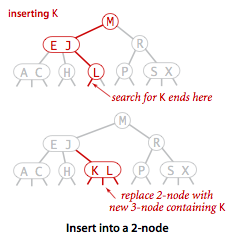
\includegraphics[width=.7\linewidth]{img/23tree-insert2.png}
 		\caption{Inserting into a 2-node.}
  		\label{fig:23tree-insert2}
	\end{subfigure}%
	\begin{subfigure}{.5\textwidth}
  		\centering
  		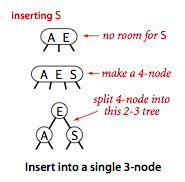
\includegraphics[width=0.5\linewidth]{img/23tree-insert3a.png}
  		\caption{Inserting into a single 3-node}
  		\label{fig:23tree-insert3a}
	\end{subfigure}
	\caption{}
	\label{fig:23tree-inserta}
\end{figure}

\begin{figure}[ht]
	\centering
	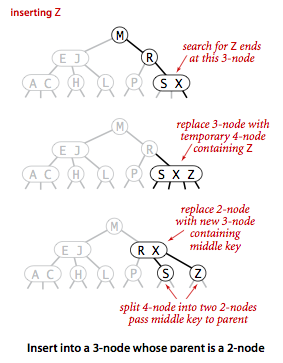
\includegraphics[scale=0.55]{img/23tree-insert3b.png}
	\caption{}
	\label{fig:23tree-insertb}
\end{figure}

\begin{figure}[ht]
	\centering
	\begin{subfigure}{.5\textwidth}
		\centering
  		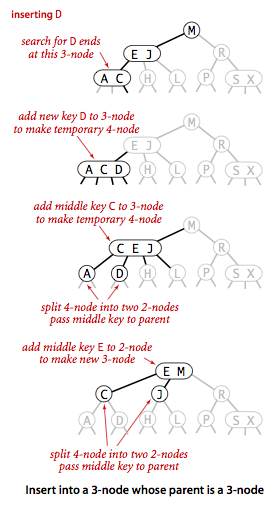
\includegraphics[width=.8\linewidth]{img/23tree-insert3c.png}
 		\caption{Insert intro a 3-node whose parent is a 3-node.}
  		\label{fig:23tree-insert3c}
	\end{subfigure}%
	\begin{subfigure}{.5\textwidth}
  		\centering
  		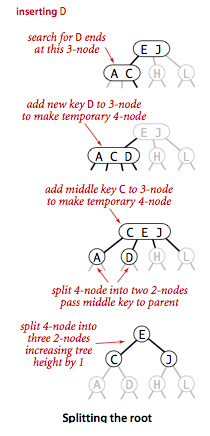
\includegraphics[width=0.6\linewidth]{img/23tree-split.png}
  		\caption{Splitting the root.}
  		\label{fig:23tree-split}
	\end{subfigure}
	\caption{}
	\label{fig:23tree-insertc}
\end{figure}

\subsubsection{Implementation}

\subsection{Hash tables}

\subsection{Summary}
The cost-summary for symbol-tables implementations is given
in table \ref{tab:cost-summary-searching}.

% auto-generated from here http://www.tablesgenerator.com/ #flemme
\begin{table}[ht]
\centering
\begin{tabular}{c|ccccc}
\multirow{2}{*}{\begin{tabular}[c]{@{}c@{}}algorithm \\(data structure)\end{tabular}} &
\multicolumn{2}{c}{\begin{tabular}[c]{@{}c@{}}worst-case cost\\ (after N inserts)\end{tabular}} &
\multicolumn{2}{c}{\begin{tabular}[c]{@{}c@{}}average-case cost\\ (after N random inserts)\end{tabular}} &
\multirow{2}{*}{\begin{tabular}[c]{@{}c@{}}efficiently support\\ordered operations?\end{tabular}} \\
                                                                                      & search                                         & insert                                         & search hit                                          & insert                                             &                                                                                                      \\ \hline
\begin{tabular}[c]{@{}c@{}}sequential search\\ (unordered linked list)\end{tabular}   & $N$                                            & $N$                                            & $N/2$                                               & $N$                                                & no                                                                                                   \\
\begin{tabular}[c]{@{}c@{}}binary search\\ (ordered array)\end{tabular}               & $\log N$                                      & $N$                                            & $\log N$                                            & $N/2$                                              & yes                                                                                                  \\
\begin{tabular}[c]{@{}c@{}}binary tree search\\ (BST)\end{tabular}                    & $N$                                            & $N$                                            & $1.39 \log N$                                       & $1.39 \log N$                                      & yes                                                                                                  \\
\begin{tabular}[c]{@{}c@{}}2-3 tree search\\ (red-black BST)\end{tabular}             & $2 \log N$                                     & $2 \log N$                                     & $1.00 \log N$                                       & $1.00 \log N$                                      & yes                                                                                                 
\end{tabular}
\caption{Cost summary for symbol-table implementations.}
\label{tab:cost-summary-searching}
\end{table}

\end{document}
